\documentclass[10pt,a4paper]{article}
\usepackage[utf8]{inputenc}
\DeclareUnicodeCharacter{00A0}{~}  % or not it by utf8x
\usepackage[T4]{fontenc}
\usepackage[polish]{babel}
%\usepackage {polski}
\let\lll\undefined
\usepackage{amssymb,amsmath,amsthm}
\usepackage[breaklinks]{hyperref}
\usepackage{graphicx}
\marginparwidth=5.2cm \hoffset=2.5cm \textwidth=12.5cm
\textheight=25.2cm \reversemarginpar \voffset=-1in
%\addtolength{\textheight}{2in}

% Moje pliki latexowe artykułów, które napisałem mają mniej więcej 1100 - 1600 słów
% i to jest trochę ponad 2 strony. A więc celuj w 1000 słów (lub 500 - na 1 stronę), a jak przekroczysz
% to nic się nie stanie. Objętość tekstu nie jest taka ważna, ważniejsza jest treść ;).

\begin{document}
%tytuł
\noindent\textbf{\LARGE Prawdopodobieństwo a informacja}

\medskip
%autor
\noindent\textit{\Large Piotr Migdał}
\marginpar{\footnotesize
    *dr z ICFO--The Institute of Photonic Sciences, Castelldefels (Barcelona), obecnie freelancer z analizy danych \url{http://migdal.wikidot.com}}

\medskip

O ile entropia jest używana w języku potocznym jako chaos i nieuporządkowanie, to sama wielkość jest ściśle określonym pojęciem --- \emph{informacją Shannona}:
%
    \marginpar{\footnotesize Częściej jest pisane w sumie $-p_i \log(p_i)$ --- równoważnie ale, moim zdaniem, mniej dydaktycznie.}
%
\begin{align}
    H = \sum_{i=1}^{n} p_i \log \left(\tfrac{1}{p_i} \right),\label{eq:entropia}
\end{align}
%
    \marginpar{\footnotesize Korzystanie z innej podstawy logarytmu, np. $e=2.718\ldots$ przemnoży wynik przez stałą, a zatem odpowiada tylko zmianie jednostek: $\ln(x)=\ln(2)\log_2(x)$. Np. dla podstawy $e$ jednostką jest \emph{nit}.}
%
gdzie $\{p_1, \ldots, p_n\}$ to pewien rozkład prawdopodobieństwa.
Będziemy używać podstawy logarytmu $2$, co odpowiada mierzeniu entropii w \emph{bitach}.
Powyższy wzór ma wiele zastosowań i interpretacji.

Ale zanim przejdziemy do nich, spójrzmy na kilka prostych przykładów.
Gdy nasz rozkład składa się z jednej możliwości, entropia wynosi $1 \log(1) = 0$ bitów --- wszak nie ma tu miejsca na losowość.
Gdy rzucamy uczciwą monetą, entropia to $\tfrac{1}{2} \log(2) + \tfrac{1}{2} \log(2) = 1$ bit.
Entropia jest największa, gdy dla ustalonej liczby zdarzeń wszystkie są równo prawdopodobne --- wtedy entropia to $\log(n)$.
Dla kostki do gry z $6$ ścianami to $\log(6)\approx 2.6$.

Warto pamiętać, że entropia jest zawsze miarą niewiedzy.
Stąd np. kostka, na której widzimy wyrzucone dwa oczka ma entropię zero.
Dowiadujemy się dokładnie tyle, o ile entropia zmalała, tu:
%
\begin{align}
    H(\tfrac{1}{6}, \tfrac{1}{6}, \tfrac{1}{6}, \tfrac{1}{6}, \tfrac{1}{6}, \tfrac{1}{6})
    - H(0, 1, 0, 0, 0, 0) = \log(6) - \log(1)
    \approx 2.6.
\end{align}
%
Gdyby ktoś nad powiedział wypadło jedno, dwa lub trzy oczka, nasz wiedza końcowa byłaby niepełna i dowiedzielibyśmy się $\log(6) - \log(3) = 1 $ bit informacji.


    \marginpar{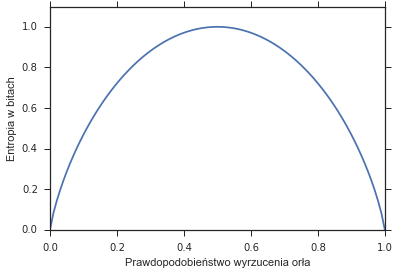
\includegraphics[height=3.5cm]{entropia2}\\
    \footnotesize Entropia rzutu obciążoną monetą.}

    % \marginpar{\footnotesize Z matematycznego punktu widzenia $\lim_{p \to 0} p \log(p) = 0$, z fizycznego --- nie chcemy by dodanie nierealistycznej opcji (tj. z zerowym prawdopodobieństwem) zmieniało wynik.}

Dlaczego potrzebujemy w tym wzorze logarytmu? 
Gdy mamy dwa niezależne zdarzenia, chcemy by ich entropia była sumą entropii składników.
Powiedzmy, że chcemy dowiedzieć się jaki jest znak zodiaku naszego obiektu westchnień oraz czy nas kocha.
Nie powinno grać roli czy dowiemy się na raz jednej informacji czy po kawałku.
Oznaczymy prawdopodobieństwa znaków zodiaku jako $\{p_1, \ldots, p_{12} \}$ oraz uczucie do nas jako $\{q_1, q_2\}$.
Tym samym prawdopodobieństwa poszczególnych, niezależnych zdarzeń to iloczyny: $p_i q_j$.
Zatem jak z entropią?
%
    \marginpar{\footnotesize Czytelnikowi, który zastanawia się czy owe dane są niezależne, polecam zapoznać się z \url{http://bit.ly/dating-zodiac}.}
%

\begin{align}
    \sum_{i=1}^{12} \sum_{j=1}^2 p_i q_j \log(1/(p_i q_j))
    &= \sum_{i=1}^{12} \sum_{j=1}^2 p_i q_j \left( \log(1/p_i) + \log(1/q_j) \right)\\
    &= \sum_{i=1}^{12} \sum_{j=1}^2 p_i q_j \log(1/p_i)
    +\sum_{i=1}^{12} \sum_{j=1}^2 p_i q_j \log(1/q_j)\\
    &= \sum_{i=1}^{12} p_i \log(1/p_i)
    + \sum_{j=1}^2 q_j \log(1/q_j),
\end{align}
%
zatem entropia niezależnych zdarzeń się dodaje.
W szczególności $n$ rzutów uczciwą monetą to $n$ bitów bitów entropii.
%
    \marginpar{\footnotesize Wnikliwy czytelnik może sprawdzić, że też $-\log \sum_{i=1}^n p_i^2$ ma tę własność.
    I ogólnie cała rodzina \emph{entropi Rényi}, będących uogólnieniem entropii Schannona;
    przy czym w ogólności nie mają one interpretacji jako informacja.}
%
Na wzór na entropię Shannona można patrzeć również jak na średnią uzyskaną informację.
Dlaczego można traktować $\log(1/p)$ jak cokolwiek związanego z informacją?
Zobaczmy to na przykładzie gry w \emph{dwadzieścia pytań}, w której jedna osoba wymyśla jakąś rzecz, a druga druga ma za zadanie zgadnąć o co chodzi, zadając po kolei pytania na `tak' lub `nie'.
Zastanawiało mnie czy warto zadawać pytania, które są z grubsza \emph{pół na pół} (np. `Czy to jest żywe?'), czy też takie w których jest niewielka szansa, że dużo się rozjaśni (np. `Czy to element biżuterii?').

Powiedzmy, że na starcie jest $m$ obiektów i każde z nich jest równoprawdopodobne.
Zadając pytanie, dla $k$ odpowiedzią jest `tak', dla pozostałych $m-k$ --- `nie'.
Wiąże się to bezpośrednio z prawdopodobieństwami odpowiedzi:
%
\begin{equation}
    p_{tak} = \tfrac{k}{m}, \qquad p_{nie} = \tfrac{m-k}{m}.
\end{equation}
%
Zatem przy nowym pytaniu pozostanie $p_{tak} \times n$ albo $p_{nie} \times n$ obiektów, w zależności od odpowiedzi.
Interesuje nas nie tyle ile uda nam się zdziałać w jednym pytaniu, ale ile w całej dwudziestce.
Skoro prawdopodobieństwa się mnożą, odpowiednią miarą jest o jaki czynnik redukujemy liczbę obiektów, które możliwym `pomyślanym' obiektem, to logarytm owej redukcji.
Zatem odpowiednią wielkością jest $\log(1/p)$, a owa średnia to:
%
\begin{equation}
    H = p_{tak} \log \left(\tfrac{1}{p_{tak}} \right) + p_{nie} \log \left(\tfrac{1}{p_{nie}} \right)
\end{equation}
%
Przy zadawaniu większej liczby pytań, o ile oczywiście możemy mieć więcej lub mniej szczęścia, to średnio logarytm z możliwości to $H_1 + \ldots + H_{q}$, i czym więcej pytań, tym nasz wynik będzie względnie bliżej średniej. 
Gdy owa wielkość dojdzie do $\log(m)$, to zredukowaliśmy możliwości do jednej, a zatem --- zgadliśmy!

Gdy zadamy pytanie `pół na pół', to niezależnie od odpowiedzi dowiadujemy się $\log(1/2)=1$ bit informacji.
A co gdy, powiedzmy, zadamy pytanie na które jest tylko $1/1000$ prawdopodobieństwo na `tak'?
Jest niewielka szansa, że dowiemy się bardzo dużo ($\log(1000)\approx 10$), ale najprawdopodobniej dowiemy się niezbyt wiele.
A sumarycznie, będzie lepiej czy gorzej? Zobaczmy!
%
\begin{equation}
    0.001 \log(\tfrac{1}{0.001}) + 0.999 \log(\tfrac{1}{0.999})\approx 0.0100 + 0.0014 = 0.0114,
\end{equation}
%
czyli bardzo niewiele!

Entropia jest też mocno związana z tym jak dobrze potrafimy skompresować dane.
Cóż, to jest treść \emph{podstawowego twierdzenia Shannona}, które mówi, że jeśli mamy ciąg liter,
każda niezależna od innych, to nie możemy średnio skompresować bardziej niż do długości $n H$.
O ile stoją za tym pewne szczegóły techniczne, główną ideę można oddać zliczając ciągi.
Liczba słów o długości $n$ nad alfabetem z $d$ literami to $d^n=2^{n \log(d)}$.
Jeśli chcielibyśmy zakodować owe słowa przy pomocy zer i jedynek,
by każde słowo miało swój kod binarnym, potrzebujemy $m = n \log(d)$ bitów.
A co jeśli nie wszystkie litery są równie często używane?
Przede wszystkim, niektóre ciągi staną się skrajnie mało prawdopodobne.
Możemy wprowadzić kody o zmiennej długości, by częstsze ciągi miały krótki kod.

Dla zwrócenia uwagi, zróbmy to na ciągu z zero i jedynek, z prawdopodobieństwami $p$ i $q$, odpowiednio.
Typowy ciąg o długości $n$ (gdzie $n$ jest duże) będzie miał $n p$ zer i $n q$ jedynek.
Prawdopodobieństwo tego ciągu to $p^{n p}q^{n q}$.
Można pokazać, że nietypowych ciągów (t.j. mających bardzo różną liczbę wystąpień zer i jedynek) jest bardzo mało.
Zatem, skoro typowe ciągi są równoprawdopodobne, liczba ich to:
$p^{-n p}q^{-n q}$.
Czyli, potrzebujemy
%
\begin{align}
    m=n \left( p \log(\tfrac{1}{p}) + q \log(\tfrac{1}{q}) \right)
\end{align}
%
bitów.
Innym słowem, liczba typowych ciągów rośnie jak $2^{n H}$.
O ile dla niewielkiego $n$ to pewne przybliżenie, to dla $n$ dążącego do nieskończoności zależność jest ścisła.

    \marginpar{\footnotesize  Lektury:\\
    Cosma Schalizi, Information theory\\
    \url{http://bactra.org/notebooks/information-theory.html}\\
    Dissecting the GZIP format\\
    \url{http://www.infinitepartitions.com/art001.html}}

Z pytań do zastanowienia się, jaką entropię mają:
\begin{itemize}
    \item ...kolejność talii 52 kart?
    \item ...litery w języku polskim?
    \item ...słowa w języku polskim?
    \item ...dwa zdarzenia, które są zależne --- większą czy mniejszą niż suma?
\end{itemize}

Oraz doświadczalne:
\begin{itemize}
    \item ...jaka jest entropia pytań w grze w dwadzieścia pytań? (do przetestowania na znajomych)?
    \item ...jaka jest efektywna wielkość przestrzeni obiektów `pomyślalnych' przez daną osobę?
\end{itemize}
I do zastanowienia się --- a co gdy ktoś myśli o rzeczach z nierównomiernym prawdopodobieństwem?


\end{document}
